\begin{activity}\label{A:0.1.3}
A simulation shows lifetime peptic ulcer rates per 100 population for different
family incomes as given in the following table.

\begin{minipage}{0.3\columnwidth}
    \begin{center}
    \begin{tabular}{|c|c|}
        \hline
        Income  & Ulcer Rate\\
        \hline \hline
        \$4000  & 14.1\\
        \$8000  & 13.4\\
        \$12000 &12.5\\
        \$16000 &12\\
        \$20000 &12.4\\
        \$24000 &11.6\\
        \$28000 &10.8\\
        \$32000 &10.3\\
        \$36000 &10.4\\
        \$40000 & 9.6\\
        \$44000 & 9.2\\
        \$48000 & 8.8\\
        \$52000 & 8.5\\
        \$56000 & 8.4\\
        \$60000 & 8.2\\ \hline
    \end{tabular}
\end{center}
\end{minipage}
\begin{minipage}{0.3\columnwidth}
    \begin{center}
        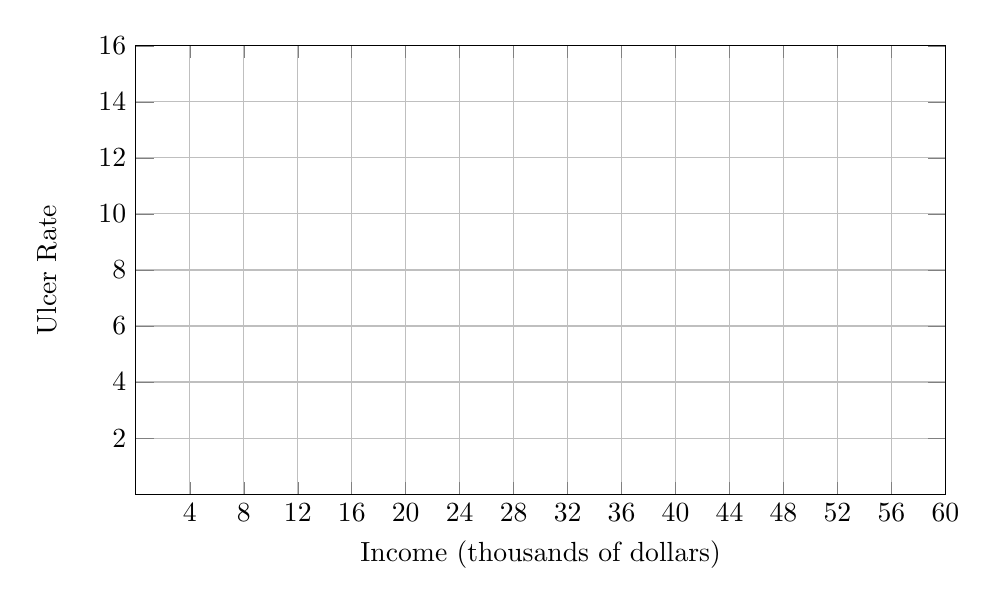
\begin{tikzpicture}
            \begin{axis}[xmin=0, xmax=60, ymin=0, ymax=16, xlabel={Income (thousands of
                dollars)}, ylabel={Ulcer Rate}, grid,
            xtick={4,8,12,16,20,24,28,32,36,40,44,48,52,56,60}, xscale=1.5,
        ytick={2,4,6,8,10,12,14,16}]
                \addplot[smooth] {0*x};
            \end{axis}
        \end{tikzpicture}
    \end{center}
\end{minipage}

This data does not represent a straight line, but it is close.
\ba 
\item Just by doing simple arithmetic, how can you tell the function is not a straight
    line?

\item Make a scatter plot of the data.  Do you think a linear model can be a good
    approximation?  Why or why not?

\item Use just the first and the last data points, what is the equation of the straight
    line that these two points determine?  Graph this equation.

\item Using the model in part (c), estimate the ulcer rate for an income of \$26000.

\item Using the model in part (c), how likely is someone with an income of \$100,000 will
    suffer from peptic ulcers?  Note your answer will be a percent and remember that the
    ulcer rate is given per 100 people of population.

\item Do you think it would be reasonable to apply this model to a person with an income
    of \$200,000?  Why or why not?
\ea
\end{activity}
\begin{smallhint}
   \ba
        \item Recall what we know about slope on a linear function.
        \item The data do not fall on one line, but are they close?
        \item It might be best to find slope first
        \item Once you have the linear function you can use it to make predictions.
        \item 
        \item
   \ea
\end{smallhint}
\begin{bighint}
   \ba
        \item
        \item
        \item
        \item
        \item
        \item
   \ea
\end{bighint}
\begin{activitySolution}
   \ba
        \item 
        \item
        \item
        \item
        \item
        \item
   \ea
\end{activitySolution}
\aftera
